\section{Gestione credenziali utenti}
Per un'agevole e rapida gestione degli utenti, essi vengono raggruppati
in gruppi. Ai gruppi possono essere attribuite particolari
proprietà (in Booked vengono chiamati ruoli) che poi verranno
riflesse agli utenti in essi contenuti, permettendogli di ampliare l'insieme
delle azioni che possono essere eseguite: I RUOLI POSSONO ESSERE MODIFICATI SOLO
DALL'APPLICATION ADMIN

\begin{figure}[H]
\centering{}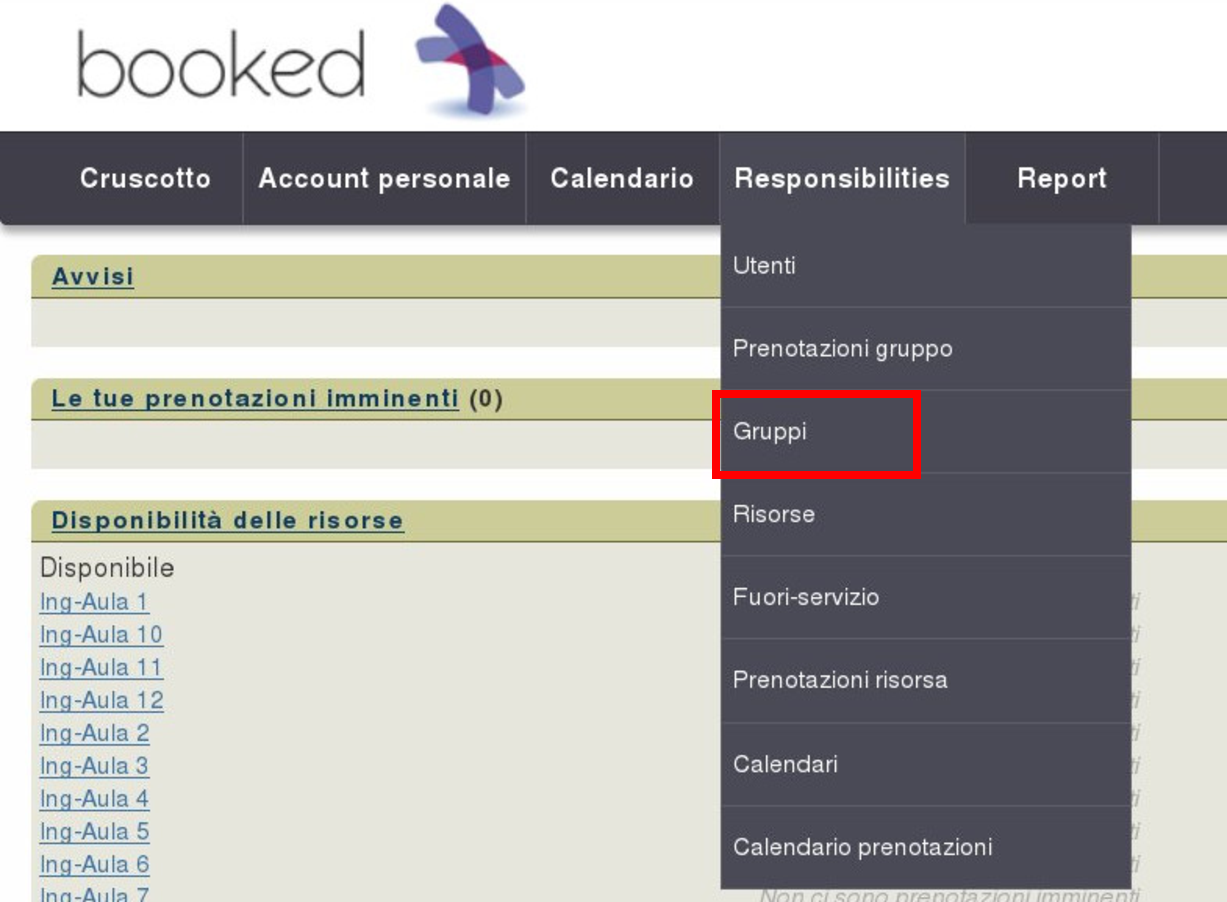
\includegraphics[scale=0.5]{Immagini/amministratore_menu_generale_selezione_gruppi.pdf}
\normalsize
\caption{}
\label{fig:amministratore_menu_generale_selezione_gruppi.pdf}
\end{figure}



\begin{figure}[H]
\centering{}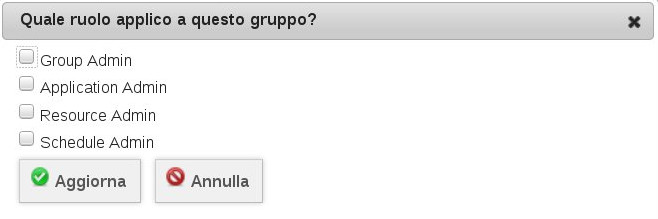
\includegraphics[scale=0.7]{Immagini/ruoli_gruppo.jpeg}
\normalsize
\caption{}
\label{fig:Ruoli assegnabili ad un gruppo}
\end{figure}

\begin{itemize}
 \item Calendar Admin (Amministratore calendario): ogni calendario ha un campo
 ``Amministratore Calendario'' dove si può scegliere uno ed un solo gruppo di utenti
 che ha la proprietà Calendar Admin attiva. Essi possono modificare le proprietà
 del calendario A, come ad esempio le fasce orarie disponibili;
 
 \item Resource Admin (Amministratore risorsa): ogni risorsa ha un campo
 ``Amministratore Risorsa'' dove si può scegliere uno ed un solo gruppo di utenti
 che ha la proprietà Resource Admin attiva. Essi potranno modificare le proprietà
 delle risorse e delle relative prentazioni,
 nonché crearne di nuove;
 
 \item Group Admin (Amministratore gruppo): ogni gruppo di utenti ha un campo
 ``Amministratore Gruppo'' dove si può scegliere uno ed un solo gruppo di utenti
 che ha la proprietà Group Admin attiva. Essi potranno modificare le proprietà
 del gruppo, come ad esempio aggiungere utenti.
 
\end{itemize}
Le proprietà (ruoli) appena elencate non sono strutturate gerarchicamente,
ma li si può abilitare uno alla volta per far sì che un utente possa effettuare
più tipi di azioni.
\paragraph*{Esempio}\mbox{}\\ %per andare a capo dopo nome paragrafo.
Il gruppo utenti con nome ``Amministratori Ingegneria'' possiede attributi Resource Admin e Calendar Admin.
L'utente Carlo fa parte di tale gruppo.
Si ha inoltre:
\begin{itemize}
 \item un calendario ``Ingegneria'' nel cui campo ``Amministratore Calendario''
 è stato impostato che il gruppo di amministratori è ``Amministratori Ingegneria'';
 \item una serie di risorse: Ing-Aula 1, Ing-Aula 2... nel cui campo
 ``Amministratore Risorsa'' è stato impostato che il gruppo di amministratori
 è ``Amministratori Ingegneria'';
\end{itemize}
perciò Carlo potrà sia modificare le risorse che i calendari di Ingegneria in quanto
il suo gruppo di appartenenza possiede le proprietà (ruoli) Resource Admin e Calendar Admin.

\paragraph*{Notare bene:}\mbox{}\\ %per andare a capo dopo nome paragrafo.
\begin{itemize}
 \item qualora il gruppo ``Amministratori Ingegneria'' non avesse avuto tra gli attributi Calendar Admin, non avrebbe potuto
essere selezionato come amministratore del calendario di Ingegneria (né ovviamente di altri);
\item qualora il gruppo ``Amministratori Ingegneria'' non avesse avuto tra gli attributi Resource Admin, non avrebbe potuto
essere selezionato come amministratore delle risorse di Ingegneria (né ovviamente di altre);
\end{itemize}